\chapter{Πειραματική Αξιολόγηση}
\label{ch:experiments}

\section{Πρωτόκολλο αξιολόγησης}
\label{sec:protocol}

Στο παρόν κεφάλαιο παρουσιάζονται και αναλύονται τα αποτελέσματα των
πειραμάτων που πραγματοποιήθηκαν για τις τρεις στρατηγικές απόσταξης
γνώσης, καθώς και η σύγκρισή τους με τα μοντέλα αναφοράς. Ως κύρια μετρική απόδοσης χρησιμοποιείται η ακρίβεια ταξινόμησης
(\tl{accuracy}) στο επίσημο σύνολο ελέγχου (\tl{test set}) του πρώτου
διαχωρισμού (\tl{split 1}) του \tl{HMDB51}
(Ενότητα~\ref{sec:hmdb51-dataset}). Ενδεικτικά, στη βιβλιογραφία έχουν καταγραφεί στο σύνολο αυτό ακρίβειες
\(73{,}3\%\) με το \tl{VideoMAE ViT-B} \cite{tong2022videomae} και
\(88{,}1\%\) με το \tl{VideoMAE V2 ViT-g} \cite{wang2023videomaev2}. Οι τιμές αυτές δεν είναι άμεσα συγκρίσιμες με τα αποτελέσματα της
παρούσας εργασίας, καθώς δεν έχουν προκύψει με το ίδιο πρωτόκολλο
προεκπαίδευσης, \tl{fine-tuning} και αξιολόγησης.

Για κάθε πείραμα αξιολογείται το
\tl{checkpoint} που επιλέχθηκε αποκλειστικά με βάση το αντίστοιχο
κριτήριο στο σύνολο επικύρωσης (\tl{validation set}), σύμφωνα με τη
διαδικασία της Ενότητας~\ref{subsec:training-settings}. Στο τέλος, τα
καλύτερα μοντέλα κάθε αρχιτεκτονικής συγκρίνονται επιπλέον ως προς τη
μείωση των παραμέτρων τους, τη μέγιστη \tl{VRAM} που απαιτούν και την
ταχύτητα επεξεργασίας (\tl{throughput}) των βίντεο κατά το
\tl{inference}, ώστε να εκτιμηθεί ο συμβιβασμός μεταξύ υπολογιστικού
κόστους και ακρίβειας.

\section{Μοντέλο-\tl{teacher} και μοντέλα αναφοράς (\tl{baselines})}
\label{sec:teacher-baseline-results} 

Πριν από την παρουσίαση των αποτελεσμάτων των στρατηγικών απόσταξης,
εξετάζονται οι επιδόσεις του μοντέλου-\tl{teacher} και των μοντέλων
αναφοράς. Το \tl{V-JEPA Large} χρησιμοποιεί το προεκπαιδευμένο
\tl{backbone} και έναν \tl{attentive classifier} εκπαιδευμένο στο
\tl{HMDB51}. Τα \tl{V-JEPA Base}, \tl{Small} και \tl{Tiny}, από την άλλη πλευρά, εκπαιδεύτηκαν από την αρχή και από άκρο σε άκρο με επιβλεπόμενο τρόπο,
χωρίς καθοδήγηση από το μοντέλο-\tl{teacher}. Τα αποτελέσματα
παρουσιάζονται στον Πίνακα~\ref{tab:baseline-results}.

\begin{table}[H]
    \centering
    \caption{Ακρίβεια ταξινόμησης στο σύνολο ελέγχου του \tl{HMDB51} για
    το μοντέλο-\tl{teacher} και τα μοντέλα αναφοράς. Η δεύτερη στήλη
    παρουσιάζει την εποχή του επιλεγμένου \tl{checkpoint} προς τον
    συνολικό αριθμό εποχών εκπαίδευσης. Το \tl{checkpoint} επιλέχθηκε με
βάση την ελάχιστη απώλεια επικύρωσης για το μοντέλο-\tl{teacher} και
τη μέγιστη ισορροπημένη ακρίβεια επικύρωσης για τα μοντέλα αναφοράς.}
    \label{tab:baseline-results}
    \small
    \begin{tabular}{lcc}
        \hline
        \textbf{Μοντέλο} & \textbf{Επιλεγμένο \tl{checkpoint}} & \textbf{\tl{Test accuracy} (\%)} \\
        \hline
        \multicolumn{3}{l}{\textit{Μοντέλο-\tl{teacher}}} \\
        \quad\tl{V-JEPA Large} & \(22/40\) & \(\mathbf{81{,}31}\) \\[6pt]
        \multicolumn{3}{l}{\textit{Μοντέλα αναφοράς}} \\
        \quad\tl{V-JEPA Base}  & \(87/100\) & \(8{,}04\)  \\
        \quad\tl{V-JEPA Small} & \(62/100\) & \(10{,}00\) \\
        \quad\tl{V-JEPA Tiny}  & \(15/100\) & \(10{,}13\) \\
        \hline
    \end{tabular}
\end{table}

Το μοντέλο-\tl{teacher} επιτυγχάνει ακρίβεια \(81{,}31\%\), η οποία
αποτελεί το ανώτερο σημείο αναφοράς για την αξιολόγηση των
μοντέλων-\tl{student}. Στόχος της απόσταξης είναι τα μικρότερα μοντέλα
να προσεγγίσουν την επίδοση αυτή με σημαντικά λιγότερες
παραμέτρους και χαμηλότερες υπολογιστικές απαιτήσεις. Όπως φαίνεται
στο Σχήμα~\ref{fig:teacher-training-curves}, κατά την εκπαίδευση του
\tl{attentive classifier} η ακρίβεια εκπαίδευσης προσεγγίζει το
\(100\%\), ενώ η ακρίβεια επικύρωσης σταθεροποιείται περίπου στο
\(80\%\). Παρότι παρατηρείται χάσμα μεταξύ των δύο καμπυλών, η επίδοση
στο σύνολο επικύρωσης παραμένει κοντά στην τελική ακρίβεια ελέγχου,
γεγονός που δείχνει ότι το προεκπαιδευμένο \tl{backbone} παράγει
αναπαραστάσεις που γενικεύουν αποτελεσματικά σε νέα βίντεο.

Ο \tl{classifier} του μοντέλου-\tl{teacher} επιλέχθηκε με βάση την
ελάχιστη απώλεια επικύρωσης, ενώ των μοντέλων-\tl{student} με βάση τη
μέγιστη ισορροπημένη ακρίβεια επικύρωσης. Για να ελεγχθεί η επίδραση
του κριτηρίου, ο \tl{classifier} του \tl{teacher} εκπαιδεύτηκε ξανά με
το δεύτερο κριτήριο. Το μοντέλο που προέκυψε επιτυγχάνει ακρίβεια
ελέγχου \(81{,}50\%\), δηλαδή μόλις \(0{,}19\) ποσοστιαίες μονάδες
υψηλότερη. Επομένως, το κριτήριο επιλογής δεν επηρεάζει ουσιαστικά τη
σύγκριση, και ως τιμή αναφοράς διατηρείται το \(81{,}31\%\).


\begin{figure}[H]
    \centering
    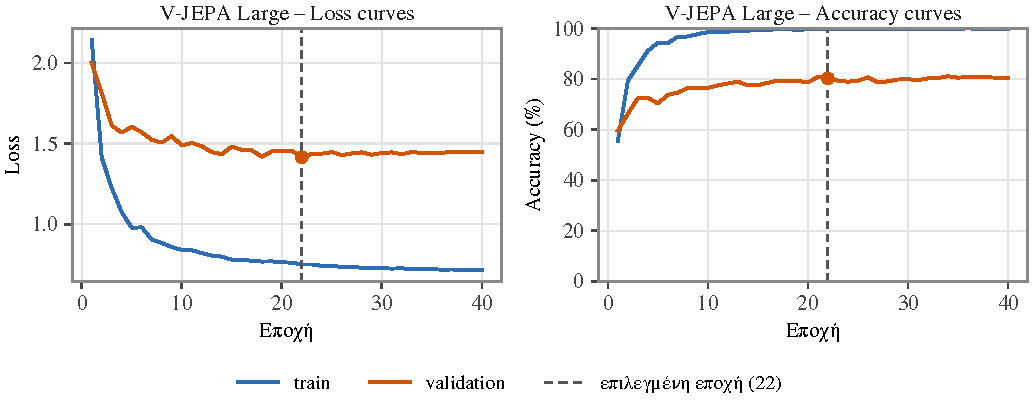
\includegraphics[width=\textwidth]{teacher_training_curves.pdf}
    \caption{Καμπύλες απώλειας και ακρίβειας κατά την επιβλεπόμενη
    εκπαίδευση του \tl{attentive classifier} πάνω στο παγωμένο
    προεκπαιδευμένο \tl{V-JEPA Large backbone}. Η κατακόρυφη γραμμή
    υποδεικνύει την επιλεγμένη εποχή, στην οποία η απώλεια επικύρωσης
    λαμβάνει την ελάχιστη τιμή της.}
    \label{fig:teacher-training-curves}
\end{figure}

Αντίθετα, τα μοντέλα αναφοράς επιτυγχάνουν ακρίβεια μεταξύ \(8\%\) και
\(10\%\). Η τιμή αυτή είναι μεν υψηλότερη από εκείνη μιας τυχαίας
πρόβλεψης, η οποία, δεδομένων των \(51\) κλάσεων του \tl{HMDB51}, θα
έβρισκε τη σωστή κλάση με πιθανότητα \(1/51 \approx 2\%\), αλλά είναι
πολύ χαμηλότερη από εκείνη του μοντέλου-\tl{teacher}.
 Οι καμπύλες εκπαίδευσής τους
(Σχήμα~\ref{fig:baseline-curves}) εμφανίζουν έντονο χάσμα μεταξύ
εκπαίδευσης και επικύρωσης. Στα \tl{V-JEPA Small} και \tl{Tiny} η
ακρίβεια εκπαίδευσης προσεγγίζει το \(100\%\), ενώ στο \tl{V-JEPA Base}
αυξάνεται πιο αργά, φτάνοντας περίπου το \(70\%\). Σε όλα τα μοντέλα,
ωστόσο, η ακρίβεια επικύρωσης παραμένει γύρω στο \(15\%\) ή χαμηλότερα και η
απώλεια επικύρωσης αυξάνεται ήδη από τις πρώτες εποχές, γεγονός που
αποτελεί σαφή ένδειξη υπερπροσαρμογής.

\begin{figure}[H]
    \centering
    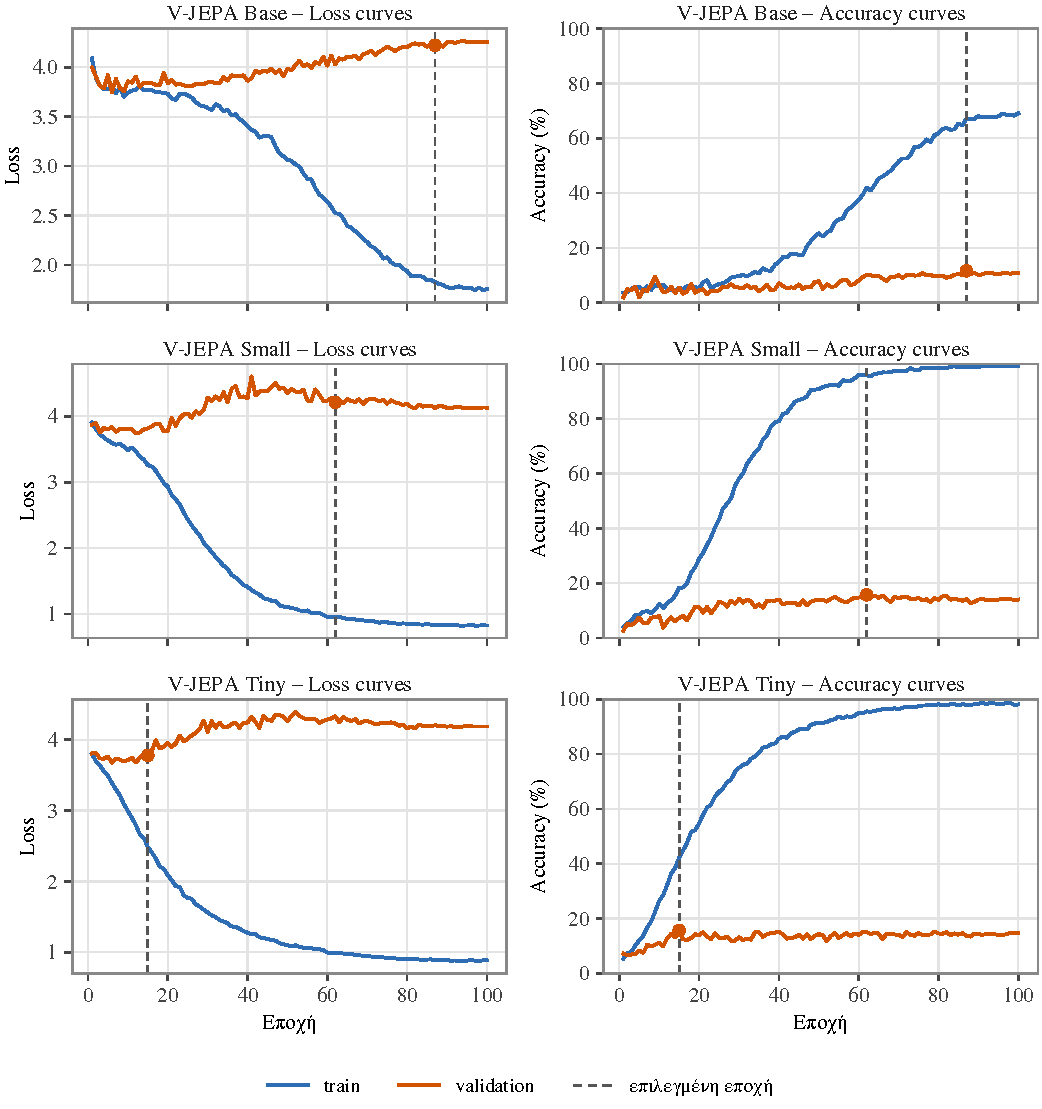
\includegraphics[width=\textwidth]{baseline_training_curves.pdf}
    \caption{Καμπύλες απώλειας και ακρίβειας κατά την επιβλεπόμενη
    εκπαίδευση των μοντέλων αναφοράς \tl{V-JEPA Base}, \tl{Small} και
    \tl{Tiny} από την αρχή στο \tl{HMDB51}. Η κατακόρυφη γραμμή υποδεικνύει
    την επιλεγμένη εποχή, στην οποία η ισορροπημένη ακρίβεια επικύρωσης
    λαμβάνει τη μέγιστη τιμή της.}

    \label{fig:baseline-curves}
\end{figure}

Η χαμηλή επίδοση των μοντέλων αναφοράς οφείλεται κυρίως στην απουσία
προεκπαίδευσης. Το μοντέλο-\tl{teacher} αξιοποιεί ένα \tl{backbone}
προεκπαιδευμένο σε μεγάλο όγκο βίντεο, ενώ τα μοντέλα αναφοράς μαθαίνουν
τις αναπαραστάσεις τους αποκλειστικά από τα περίπου \(2.900\) δείγματα
του συνόλου εκπαίδευσης του \tl{HMDB51}. Καθώς οι αρχιτεκτονικές
\tl{Vision Transformer} απαιτούν συνήθως μεγάλο όγκο δεδομένων όταν
εκπαιδεύονται από την αρχή \cite{dosovitskiy2021image}, το περιορισμένο
αυτό σύνολο οδηγεί στην υπερπροσαρμογή που παρατηρείται στις καμπύλες
εκπαίδευσης. Επομένως, η επιβλεπόμενη εκπαίδευση των συγκεκριμένων
αρχιτεκτονικών από την αρχή δεν αποτελεί αποτελεσματική λύση για την
εργασία αναγνώρισης ενεργειών στο \tl{HMDB51}. Οι επιδόσεις των μοντέλων
αναφοράς αποτελούν, έτσι, το κάτω όριο σύγκρισης για τα
μοντέλα-\tl{student} των επόμενων ενοτήτων, επιτρέποντας την εκτίμηση
του οφέλους που προκύπτει από την απόσταξη γνώσης.

\section{Απόσταξη τελικών προβλέψεων}
\label{sec:logit-kd-results}

\begin{table}[H]
    \centering
    \caption{Ακρίβεια ταξινόμησης στο σύνολο ελέγχου του \tl{HMDB51} για
    τα μοντέλα-\tl{student} που εκπαιδεύτηκαν με απόσταξη τελικών
    προβλέψεων. Σε όλα τα πειράματα χρησιμοποιείται η απώλεια \tl{KL}
    με παράμετρο θερμοκρασίας \(T=1\). Η δεύτερη στήλη δηλώνει
    αν εφαρμόστηκε \tl{mixup}.}
    \label{tab:logit-kd-results}
    \small
    \begin{tabular}{lccc}
        \hline
        \textbf{Μοντέλο-\tl{student}} & \textbf{\tl{Mixup}} & \textbf{Επιλεγμένη εποχή} & \textbf{\tl{Test accuracy} (\%)} \\
        \hline
        \tl{V-JEPA Base}  & Όχι & \(80/100\) & \(11{,}57\) \\
        \tl{V-JEPA Small} & Όχι & \(37/100\) & \(12{,}68\) \\
        \tl{V-JEPA Tiny}  & Όχι & \(18/100\) & \(11{,}96\) \\
        \tl{V-JEPA Tiny}  & Ναι & \(97/100\) & \(\mathbf{16{,}99}\) \\
        \hline
    \end{tabular}
\end{table}

Τα αποτελέσματα του Πίνακα~\ref{tab:logit-kd-results} δείχνουν
περιορισμένη βελτίωση σε σχέση με τα μοντέλα αναφοράς. Χωρίς
\tl{mixup}, η ακρίβεια αυξάνεται κατά \(3{,}53\), \(2{,}68\) και
\(1{,}83\) ποσοστιαίες μονάδες για τα \tl{V-JEPA Base}, \tl{Small} και
\tl{Tiny}, αντίστοιχα. Αυτό υποδεικνύει ότι η πληροφορία των τελικών κατανομών πιθανοτήτων
του μοντέλου-\tl{teacher} δεν επαρκεί για να μάθουν μικρότερα μοντέλα,
εκπαιδευόμενα από την αρχή, αναπαραστάσεις που γενικεύουν. Τη μεγαλύτερη βελτίωση φέρνει το \tl{mixup}, το οποίο εφαρμόστηκε
ενδεικτικά στο \tl{V-JEPA Tiny} και αυξάνει την ακρίβεια του κατά περίπου
\(5\) ποσοστιαίες μονάδες.

\begin{figure}[H]
    \centering
    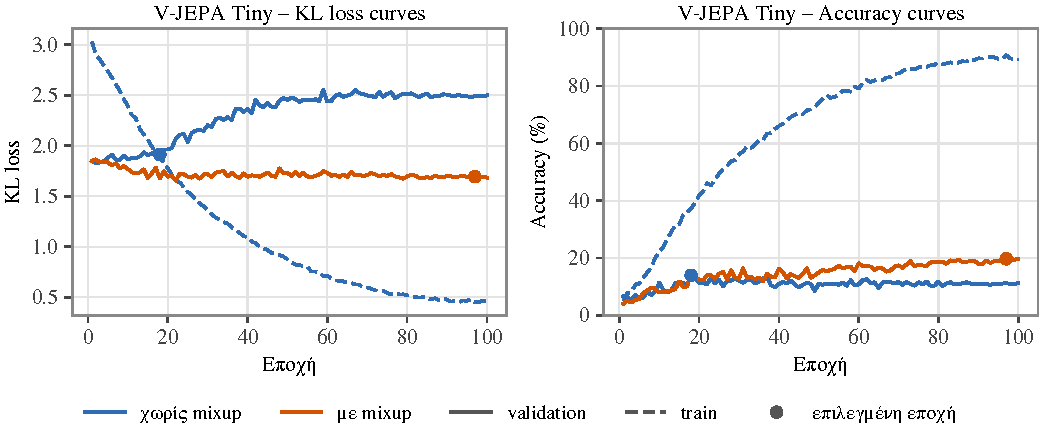
\includegraphics[width=\textwidth]{logit_kd_tiny_curves.pdf}
    \caption{Καμπύλες απώλειας \tl{KL} και ακρίβειας κατά την απόσταξη
    τελικών προβλέψεων στο \tl{V-JEPA Tiny}, χωρίς και με \tl{mixup}.
            Με \tl{mixup} παρουσιάζονται μόνο οι καμπύλες επικύρωσης, καθώς τα
    δείγματα εκπαίδευσης είναι ανάμειξη δύο βίντεο, οπότε η ακρίβεια
    εκπαίδευσης δεν έχει σαφή ερμηνεία και η απώλεια εκπαίδευσης δεν
    συγκρίνεται άμεσα με εκείνη της επικύρωσης. Οι κουκκίδες
    υποδεικνύουν την εποχή του \tl{checkpoint} που επιλέχθηκε με βάση τη
    μέγιστη ακρίβεια επικύρωσης.}
    \label{fig:logit-kd-curves}
\end{figure}

Οι καμπύλες του Σχήματος~\ref{fig:logit-kd-curves} εξηγούν τη βελτίωση
που προσφέρει το \tl{mixup}. Χωρίς αυτό, η ακρίβεια εκπαίδευσης φτάνει περίπου το
\(90\%\), ενώ η απώλεια επικύρωσης αυξάνεται μετά τις πρώτες εποχές,
γεγονός που δείχνει υπερπροσαρμογή. Με \tl{mixup}, η απώλεια επικύρωσης παραμένει σχετικά σταθερή και η
ακρίβεια επικύρωσης βελτιώνεται σταδιακά σχεδόν μέχρι το τέλος της
εκπαίδευσης. Η συμπεριφορά αυτή αποτελεί ένδειξη ότι το \tl{mixup}
περιορίζει την υπερπροσαρμογή, λειτουργώντας ως μέθοδος
κανονικοποίησης (\tl{regularization}). Για τον λόγο αυτό, το \tl{mixup} εφαρμόστηκε και στις επόμενες
στρατηγικές απόσταξης. Επειδή όμως η ακρίβεια παρέμεινε χαμηλή, η
στρατηγική απόσταξης αυτή δεν διερευνήθηκε περαιτέρω και η μελέτη στράφηκε σε
στρατηγικές που αξιοποιούν και τις ενδιάμεσες αναπαραστάσεις του
μοντέλου-\tl{teacher}.

\section{Υβριδική απόσταξη γνώσης}
\label{sec:hybrid-kd-results}

\subsection{Διερεύνηση των υπερπαραμέτρων}
\label{subsec:hybrid-kd-hyperparameters}

\begin{table}[H]
    \centering
    \caption{Ακρίβεια ταξινόμησης στο σύνολο ελέγχου του \tl{HMDB51} για
    τα μοντέλα-\tl{student} που εκπαιδεύτηκαν με υβριδική απόσταξη. Σε
    όλα τα πειράματα χρησιμοποιούνται \tl{mixup}, γραμμικός προβολέας
    και συντελεστής βαρύτητας της απώλειας \tl{KL} \(\lambda_{\mathrm{KL}}=1\),
   ενώ \(\ell\) είναι η συνάρτηση που
    χρησιμοποιείται στην απώλεια αναπαραστάσεων \(\mathcal{L}_{\mathrm{feat}}\)
    (Εξίσωση~\eqref{eq:feat-loss}). Η πρώτη ομάδα αφορά τη διερεύνηση
    των υπερπαραμέτρων στο \tl{V-JEPA Small} και η δεύτερη την εφαρμογή της ίδιας διαμόρφωσης και 
    στα τρία μοντέλα, για τη σύγκριση των αρχιτεκτονικών.}
    \label{tab:hybrid-kd-results}
    \small
    \begin{tabular}{lccccc}
        \hline
        \textbf{Μοντέλο-\tl{student}} & \(\boldsymbol{\ell}\) &
        \(\boldsymbol{\lambda_{\mathrm{feat}}}\) & \(\boldsymbol{T}\) &
        \textbf{Επιλεγμένη εποχή} & \textbf{\tl{Test accuracy} (\%)} \\
        \hline
        \multicolumn{6}{l}{\textit{Διερεύνηση υπερπαραμέτρων}} \\
        \quad\tl{V-JEPA Small} & \tl{MSE}      & \(1\) & \(1\) & \(63/80\)   & \(18{,}69\) \\
        \quad\tl{V-JEPA Small} & \tl{SmoothL1} & \(1\) & \(1\) & \(70/80\)   & \(16{,}54\) \\
        \quad\tl{V-JEPA Small} & \tl{SmoothL1} & \(1\) & \(1\) & \(88/120\)  & \(17{,}78\) \\
        \quad\tl{V-JEPA Small} & \tl{MSE}      & \(3\) & \(1\) & \(117/120\) & \(26{,}67\) \\
        \quad\tl{V-JEPA Small} & \tl{MSE}      & \(3\) & \(2\) & \(110/120\) & \(33{,}79\) \\
        \quad\tl{V-JEPA Small} & \tl{MSE}      & \(3\) & \(1\) & \(158/160\) & \(28{,}17\) \\[6pt]
         \multicolumn{6}{l}{\textit{Κοινή διαμόρφωση για τις τρεις αρχιτεκτονικές}} \\
        \quad\tl{V-JEPA Base}  & \tl{MSE}      & \(3\) & \(2\) & \(154/160\) & \(\mathbf{37{,}65}\) \\
        \quad\tl{V-JEPA Small} & \tl{MSE}      & \(3\) & \(2\) & \(154/160\) & \(34{,}77\) \\
        \quad\tl{V-JEPA Tiny}  & \tl{MSE}      & \(3\) & \(2\) & \(159/160\) & \(29{,}67\) \\
        \hline
    \end{tabular}
\end{table}

\begin{figure}[H]
    \centering
    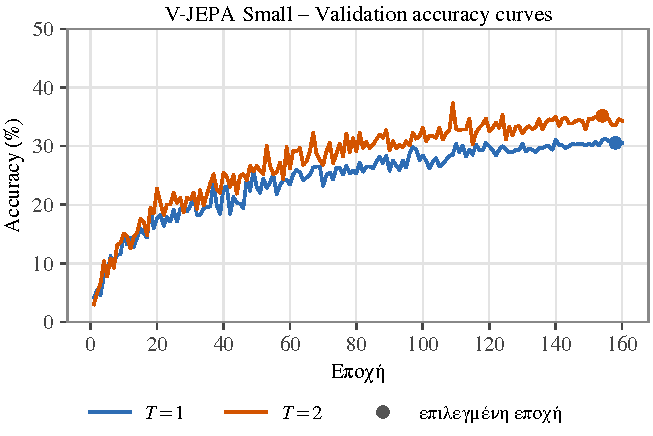
\includegraphics[width=0.65\textwidth]{hybrid_kd_temperature_curves.pdf}
    \caption{Ακρίβεια επικύρωσης για το μοντέλο-\tl{student} \tl{V-JEPA Small} με υβριδική απόσταξη για
    παραμέτρους θερμοκρασίας \(T=1\) και \(T=2\), απώλεια αναπαραστάσεων \tl{MSE} με συντελεστή βαρύτητας \(\lambda_{\mathrm{feat}}=3\) και
    \(160\) εποχές εκπαίδευσης. Οι
    κουκκίδες υποδεικνύουν την εποχή του \tl{checkpoint} που επιλέχθηκε
    με βάση την ελάχιστη συνολική απώλεια επικύρωσης.}
    \label{fig:hybrid-temperature-curves}
\end{figure}

Η διερεύνηση των υπερπαραμέτρων (Πίνακας~\ref{tab:hybrid-kd-results})
δείχνει αρχικά ότι ο συνδυασμός της
\tl{MSE} με την απώλεια \tl{KL} αποδίδει καλύτερα από τον αντίστοιχο
συνδυασμό \tl{SmoothL1} και \tl{KL}. Στο \tl{V-JEPA Small}, η
\tl{MSE} επιτυγχάνει ακρίβεια \(18{,}69\%\) έπειτα από \(80\) εποχές,
ενώ η \tl{SmoothL1} φτάνει το \(16{,}54\%\) για τον ίδιο αριθμό εποχών
και το \(17{,}78\%\) ακόμη και όταν η εκπαίδευση επεκτείνεται στις
\(120\) εποχές. Επιπλέον, η αύξηση της βαρύτητας της απώλειας
αναπαραστάσεων σε \(\lambda_{\mathrm{feat}}=3\), σε συνδυασμό με
μεγαλύτερη διάρκεια εκπαίδευσης, βελτιώνει περαιτέρω την ακρίβεια.
Τέλος, η αύξηση της παραμέτρου θερμοκρασίας σε \(T=2\) οδηγεί σε πρόσθετη
βελτίωση τόσο στις \(120\) όσο και στις \(160\) εποχές. Όπως φαίνεται στο
Σχήμα~\ref{fig:hybrid-temperature-curves}, η διαφορά αυτή γίνεται περισσότερο εμφανής μετά τις πρώτες \(50\)
περίπου εποχές και διατηρείται μέχρι το τέλος της εκπαίδευσης. 

Με βάση τα αποτελέσματα αυτά, η διαμόρφωση με \tl{MSE},
\(\lambda_{\mathrm{feat}}=3\), \(T=2\), \(160\) εποχές και γραμμικό
προβολέα χρησιμοποιήθηκε ως κοινή βάση για τη σύγκριση των τριών
αρχιτεκτονικών. Σε σχέση με την απόσταξη μόνο των τελικών προβλέψεων, η
υβριδική απόσταξη αυξάνει την ακρίβεια κατά \(26{,}08\) και \(22{,}09\)
ποσοστιαίες μονάδες για τα \tl{V-JEPA Base} και \tl{Small}, αντίστοιχα.
Για το \tl{V-JEPA Tiny}, η βελτίωση είναι \(12{,}68\) ποσοστιαίες
μονάδες σε σχέση με την απόσταξη τελικών προβλέψεων με \tl{mixup}, η
οποία είχε ήδη βελτιώσει την επίδοσή του στην πρώτη στρατηγική.


\subsection{Επίδραση της διαμόρφωσης του προβολέα}
\label{subsec:hybrid-kd-projectors}

\begin{table}[H]
    \centering
    \caption{Ακρίβεια ταξινόμησης στο σύνολο ελέγχου του \tl{HMDB51} για
    το \tl{V-JEPA Base} με διαφορετικές διαμορφώσεις του προβολέα. Σε
    όλα τα πειράματα χρησιμοποιούνται \tl{mixup}, απώλεια αναπαραστάσεων
    \tl{MSE}, \(\lambda_{\mathrm{feat}}=3\), \(\lambda_{\mathrm{KL}}=1\) και \(T=2\).}
    \label{tab:hybrid-projectors}
    \small
    \begin{tabular}{lcc}
        \hline
        \textbf{Προβολέας} & \textbf{Επιλεγμένη εποχή} & \textbf{\tl{Test accuracy} (\%)} \\
        \hline
        Γραμμικός                      & \(154/160\) & \(37{,}65\) \\
        Γραμμικός με \tl{LayerNorm}    & \(159/160\) & \(\mathbf{41{,}50}\) \\
        Μη γραμμικός                   & \(159/160\) & \(38{,}17\) \\
        Αντίστροφη προβολή             & \(99/160\)  & \(14{,}97\) \\
        \hline
    \end{tabular}
\end{table}

\begin{figure}[H]
    \centering
    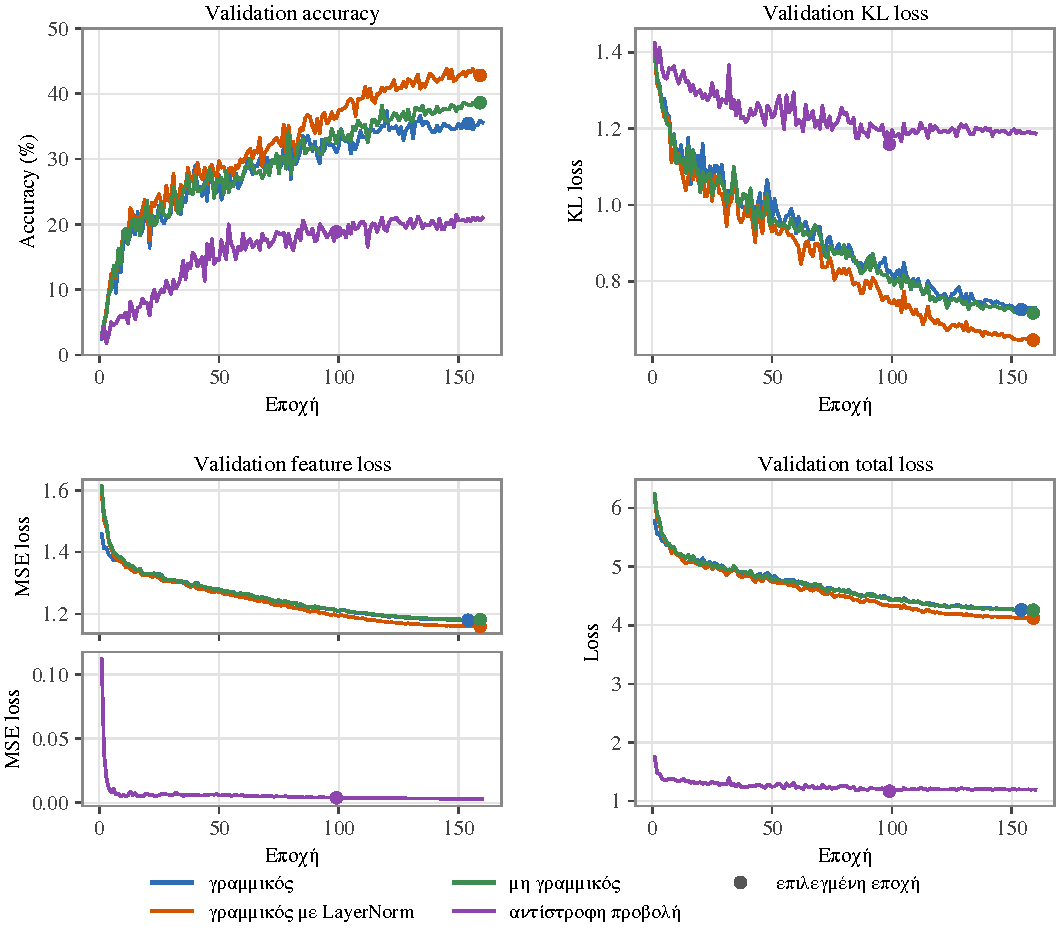
\includegraphics[width=\textwidth]{hybrid_kd_projector_curves.pdf}
    \caption{Σύγκριση ακρίβειας, απώλειας \tl{KL}, απώλειας αναπαραστάσεων
    \tl{MSE} και συνολικής απώλειας στο σύνολο επικύρωσης του
    \tl{V-JEPA Base} για διαφορετικές διαμορφώσεις του προβολέα. Οι
    κουκκίδες υποδεικνύουν την επιλεγμένη εποχή, στην οποία η συνολική
    απώλεια επικύρωσης λαμβάνει την ελάχιστη τιμή της.}
    \label{fig:hybrid-projector-curves}
\end{figure}

Στο \tl{V-JEPA Base} (Πίνακας~\ref{tab:hybrid-projectors},
Σχήμα~\ref{fig:hybrid-projector-curves}), η προσθήκη \tl{LayerNorm} μετά τη γραμμική προβολή υπερέχει στο
σύνολο επικύρωσης, καθώς από την \(80\)ή περίπου εποχή επιτυγχάνει
υψηλότερη ακρίβεια και χαμηλότερη απώλεια \tl{KL} από τους υπόλοιπους
προβολείς. Η υπεροχή αυτή
επιβεβαιώνεται και στο σύνολο ελέγχου, όπου η ακρίβεια αυξάνεται από
\(37{,}65\%\) σε \(41{,}50\%\), δηλαδή κατά περίπου \(4\) ποσοστιαίες
μονάδες. Αντίθετα, ο μη γραμμικός προβολέας παρουσιάζει σχεδόν ίδιες
απώλειες επικύρωσης με τον απλό γραμμικό προβολέα, ενώ η ακρίβειά του
στο σύνολο ελέγχου (\(38{,}17\%\)) είναι επίσης παρόμοια. Επομένως, η
πρόσθετη πολυπλοκότητά του δεν προσφέρει ουσιαστικό όφελος.

Η αντίστροφη προβολή οδηγεί σε σημαντική πτώση της ακρίβειας. Παρότι η
απώλεια αναπαραστάσεων μειώνεται σχεδόν στο μηδέν, αυτό δεν αντιστοιχεί
σε αποτελεσματικότερη μεταφορά γνώσης. Καθώς ο εκπαιδεύσιμος προβολέας
εφαρμόζεται στις αναπαραστάσεις του \tl{teacher}, ο στόχος της
απόσταξης δεν παραμένει σταθερός, αλλά μεταβάλλεται κατά την εκπαίδευση.
Έτσι, ο προβολέας μπορεί να προσαρμόζει τον στόχο και να μειώνει την
απώλεια, χωρίς ο \tl{student} να μαθαίνει αναπαραστάσεις που διατηρούν
την πληροφορία του \tl{teacher}, οδηγώντας σε μια εκφυλισμένη λύση
(\tl{degenerate solution}). Ο όρος αναπαραστάσεων παύει επομένως να
παρέχει ουσιαστική καθοδήγηση, αφήνοντας τον όρο \tl{KL} ως τον μόνο
σταθερό στόχο εκπαίδευσης. Σε συμφωνία με την ερμηνεία αυτή, η απώλεια
\tl{KL} παραμένει υψηλότερη από ό,τι με τους υπόλοιπους προβολείς, ενώ
η ακρίβεια βρίσκεται κοντά σε εκείνη της απόσταξης μόνο των τελικών
προβλέψεων (Ενότητα~\ref{sec:logit-kd-results}). Το αποτέλεσμα αυτό
υποδεικνύει ότι, κατά την απόσταξη αναπαραστάσεων, ο στόχος πρέπει να
προκύπτει απευθείας από τις αναπαραστάσεις του \tl{teacher}, χωρίς να
μεταβάλλεται από εκπαιδεύσιμες παραμέτρους.


Συνολικά, η υβριδική απόσταξη βελτιώνει σημαντικά την επίδοση των
μοντέλων-\tl{student} σε σχέση τόσο με τα μοντέλα αναφοράς όσο και με
την απόσταξη μόνο των τελικών προβλέψεων. Αυτό δείχνει ότι οι αναπαραστάσεις που παράγει το \tl{backbone}
 του μοντέλου-\tl{teacher} παρέχουν
χρήσιμη πρόσθετη πληροφορία για την εκπαίδευση των μικρότερων
μοντέλων. Ωστόσο, ακόμη και το καλύτερο μοντέλο της στρατηγικής, το
\tl{V-JEPA Base} με γραμμικό προβολέα και \tl{LayerNorm}
(\(41{,}50\%\)), παραμένει μακριά από την ακρίβεια του
μοντέλου-\tl{teacher} (\(81{,}31\%\)), ενώ η απόσταση είναι ακόμη
μεγαλύτερη για τις μικρότερες αρχιτεκτονικές \tl{V-JEPA Small} και
\tl{Tiny}. Καθώς η διερεύνηση επικεντρώθηκε στη
συνέχεια στην τρίτη στρατηγική απόσταξης, οι διαφορετικές διαμορφώσεις
του προβολέα δεν εξετάστηκαν στα μοντέλα αυτά.

\section{Απόσταξη του \tl{backbone}}
\label{sec:backbone-kd}

\subsection{Διερεύνηση της πειραματικής διαμόρφωσης}
\label{subsec:backbone-kd-exploration}

\begin{table}[H]
    \centering
    \caption{Αποτελέσματα στο
    \tl{HMDB51} κατά τη διερεύνηση της διαμόρφωσης της απόσταξης του
    \tl{backbone}. Σε όλα τα πειράματα η απόσταξη πραγματοποιείται στο
    \tl{HMDB51} για \(80\) εποχές με γραμμικό προβολέα. Οι επαυξήσεις
    του \tl{classifier} αντιστοιχούν σε \tl{Random Resized Crop} και
    \tl{Random Horizontal Flip}.}
    \label{tab:backbone-kd-exploration}
    \small
    \setlength{\tabcolsep}{4pt}
    \begin{tabular}{lccccc}
        \hline
        \begin{tabular}[c]{@{}l@{}}\textbf{Μοντέλο}\\\textbf{\tl{student}}\end{tabular} &
        \begin{tabular}[c]{@{}c@{}}\textbf{\tl{Backbone}}\\\textbf{\tl{mixup}}\end{tabular} &
        \(\boldsymbol{\ell}\) &
        \begin{tabular}[c]{@{}c@{}}\textbf{\tl{Classifier}}\\\textbf{\tl{augmentations}}\end{tabular} &
        \begin{tabular}[c]{@{}c@{}}\textbf{\tl{Val. balanced}}\\\textbf{\tl{accuracy} (\%)}\end{tabular} &
        \begin{tabular}[c]{@{}c@{}}\textbf{\tl{Test}}\\\textbf{\tl{accuracy} (\%)}\end{tabular} \\
        \hline
        \tl{V-JEPA Tiny}  & Ναι & \tl{MSE}      & Όχι & \(41{,}84\) & \(38{,}50\) \\
        \tl{V-JEPA Small} & Όχι & \tl{MSE}      & Όχι & \(53{,}41\) & \(51{,}57\) \\
        \tl{V-JEPA Small} & Ναι & \tl{MSE}      & Όχι & \(56{,}26\) & \(53{,}27\) \\
        \tl{V-JEPA Base}  & Ναι & \tl{MSE}      & Όχι & \(64{,}98\) & \(64{,}90\) \\
        \tl{V-JEPA Base}  & Ναι & \tl{MSE}      & Ναι & \(64{,}43\) & \(63{,}66\) \\
        \tl{V-JEPA Base}  & Ναι & \tl{SmoothL1} & Ναι & \(\mathbf{66{,}96}\) & \(\mathbf{66{,}14}\) \\
        \hline
    \end{tabular}
\end{table}

Τα αποτελέσματα της διερεύνησης
(Πίνακας~\ref{tab:backbone-kd-exploration}) δείχνουν ότι, ήδη με
\(80\) εποχές απόσταξης, η στρατηγική αυτή υπερέχει σημαντικά των δύο
προηγούμενων. Το \tl{V-JEPA Base} υπερβαίνει την υβριδική απόσταξη με
\(160\) εποχές κατά \(28{,}49\) ποσοστιαίες μονάδες. Η χρήση \tl{mixup} κατά την απόσταξη αυξάνει
την ακρίβεια του \tl{V-JEPA Small} κατά \(1{,}70\) ποσοστιαίες μονάδες,
αναδεικνύοντας για ακόμη μία φορά τη συμβολή της στην εκπαίδευση. Σε
αντίθεση με την υβριδική στρατηγική, η απώλεια \tl{SmoothL1} αποδίδει
καλύτερα από τη \tl{MSE}, με βελτίωση \(2{,}48\) ποσοστιαίων μονάδων
για το \tl{V-JEPA Base}. Αντίθετα, οι επαυξήσεις κατά την εκπαίδευση
του \tl{attentive classifier} δεν οδηγούν σε βελτίωση, καθώς η
ακρίβεια μειώνεται κατά \(1{,}24\) μονάδες. Οι ίδιες τάσεις παρατηρούνται και
στην ισορροπημένη ακρίβεια επικύρωσης, με βάση την οποία επιλέχθηκε η
διαμόρφωση των επόμενων πειραμάτων. Η συμπεριφορά του ταξινομητή και το φαινόμενο της
υπερπροσαρμογής εξετάζονται αναλυτικότερα στην
Ενότητα~\ref{subsec:backbone-kd-overfitting}.

\subsection{Επίδραση της διάρκειας και των δεδομένων απόσταξης}
\label{subsec:backbone-kd-epochs-data}

\begin{table}[H]
    \centering
    \caption{Αποτελέσματα στο
\tl{HMDB51} μετά από \(200\) και \(300\) εποχές απόσταξης του
\tl{backbone}. Σε όλα τα πειράματα χρησιμοποιούνται \tl{mixup}, απώλεια
\tl{SmoothL1} και \tl{data augmentations} κατά την εκπαίδευση του
\tl{attentive classifier}. Στις δύο πρώτες ομάδες χρησιμοποιείται
γραμμικός προβολέας, ενώ στην τελευταία προστίθεται \tl{LayerNorm}.}
    \label{tab:backbone-kd-results}
    \small
    \begin{tabular}{lcc}
        \hline
        \textbf{Μοντέλο-\tl{student}} &
        \begin{tabular}[c]{@{}c@{}}\textbf{\tl{Val. balanced}}\\\textbf{\tl{accuracy} (\%)}\end{tabular} &
        \begin{tabular}[c]{@{}c@{}}\textbf{\tl{Test}}\\\textbf{\tl{accuracy} (\%)}\end{tabular} \\
        \hline
        \multicolumn{3}{l}{\textit{\(200\) εποχές απόσταξης}} \\
        \quad\tl{V-JEPA Base}  & \(74{,}21\) & \(74{,}25\) \\
        \quad\tl{V-JEPA Small} & \(66{,}83\) & \(66{,}21\) \\
        \quad\tl{V-JEPA Tiny}  & \(53{,}62\) & \(50{,}52\) \\[6pt]
        \multicolumn{3}{l}{\textit{\(300\) εποχές απόσταξης}} \\
        \quad\tl{V-JEPA Base}  & \(\mathbf{75{,}24}\) & \(\mathbf{75{,}62}\) \\
        \quad\tl{V-JEPA Small} & \(68{,}97\) & \(68{,}17\) \\
        \quad\tl{V-JEPA Tiny}  & \(56{,}58\) & \(54{,}25\) \\[6pt]
        \multicolumn{3}{l}{\textit{Προβολέας με \tl{LayerNorm}, \(200\) εποχές}} \\
        \quad\tl{V-JEPA Base}  & \(74{,}18\) & \(75{,}16\) \\
        \hline
    \end{tabular}
\end{table}

\begin{figure}[H]
    \centering
    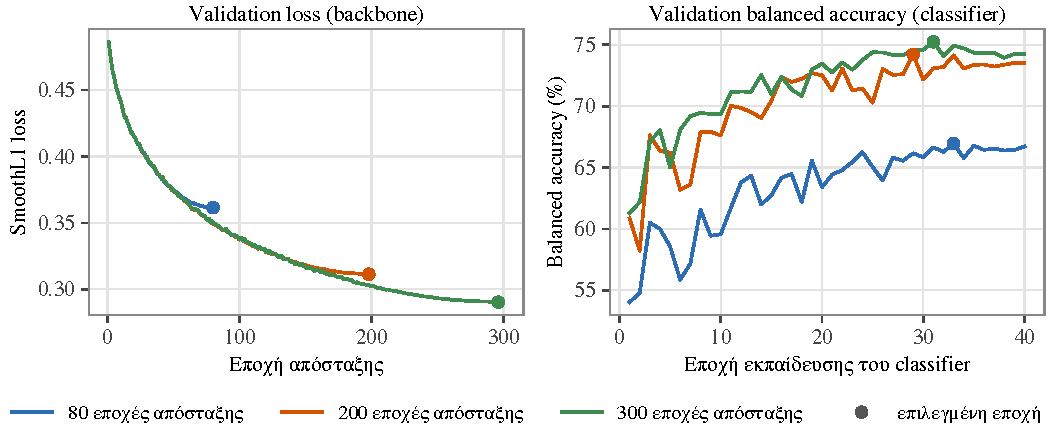
\includegraphics[width=\textwidth]{backbone_kd_epochs_curves.pdf}
   \caption{Επίδραση του αριθμού των εποχών απόσταξης στο
\tl{V-JEPA Base}, με χρήση του \tl{HMDB51}. Αριστερά παρουσιάζεται η
απώλεια επικύρωσης \tl{SmoothL1} κατά την απόσταξη του \tl{backbone}
για \(80\), \(200\) και \(300\) εποχές. Δεξιά παρουσιάζεται η
ισορροπημένη ακρίβεια επικύρωσης κατά την εκπαίδευση του
\tl{attentive classifier} με το αντίστοιχο αποσταγμένο \tl{backbone}.
Οι κουκκίδες υποδεικνύουν τις επιλεγμένες εποχές, στις οποίες η
απώλεια επικύρωσης της απόσταξης λαμβάνει την ελάχιστη τιμή της και η
ισορροπημένη ακρίβεια επικύρωσης τη μέγιστη τιμή της, αντίστοιχα.}
    \label{fig:backbone-kd-epochs-curves}
\end{figure}

Η αύξηση της διάρκειας της απόσταξης βελτιώνει σημαντικά την ακρίβεια
(Πίνακες~\ref{tab:backbone-kd-exploration} και~\ref{tab:backbone-kd-results}). Για το \tl{V-JEPA Base}, η
αύξηση από \(80\) σε \(200\) εποχές βελτιώνει την ακρίβεια κατά
\(8{,}11\) ποσοστιαίες μονάδες. Όπως φαίνεται στο
Σχήμα~\ref{fig:backbone-kd-epochs-curves}, η μεγαλύτερη διάρκεια
οδηγεί σε χαμηλότερη απώλεια επικύρωσης της απόσταξης, γεγονός που
αντανακλάται και σε υψηλότερη ακρίβεια επικύρωσης του
\tl{attentive classifier}. Η περαιτέρω αύξηση σε \(300\) εποχές
βελτιώνει την ακρίβεια και των τριών μοντέλων, κατά \(1{,}37\),
\(1{,}96\) και \(3{,}73\) ποσοστιαίες μονάδες για τα \tl{V-JEPA Base},
\tl{Small} και \tl{Tiny}, αντίστοιχα, με το όφελος να είναι μικρότερο
από εκείνο της μετάβασης από \(80\) σε \(200\) εποχές.

Επιπλέον, εξετάστηκε και ο γραμμικός προβολέας με \tl{LayerNorm}, ο οποίος
είχε βελτιώσει την ακρίβεια στην υβριδική στρατηγική. Στην περίπτωση
αυτή, ωστόσο, δεν προσφέρει ουσιαστική βελτίωση: η ισορροπημένη
ακρίβεια επικύρωσης είναι σχεδόν ίδια (\(74{,}18\%\) έναντι
\(74{,}21\%\)) και η ακρίβεια ελέγχου διαφέρει κατά \(0{,}91\)
ποσοστιαίες μονάδες. Για τον λόγο αυτό, στα υπόλοιπα πειράματα
διατηρήθηκε ο απλός γραμμικός προβολέας.

\begin{table}[H]
    \centering
    \caption{Αποτελέσματα του \tl{V-JEPA Base} στο \tl{HMDB51} για διαφορετικά σύνολα δεδομένων απόσταξης
    (Ενότητα~\ref{sec:dataset-usage}). Σε όλα τα πειράματα ο
    \tl{attentive classifier} εκπαιδεύεται και αξιολογείται στο
    \tl{HMDB51}, ενώ οι υπόλοιπες ρυθμίσεις της απόσταξης και του
    \tl{classifier} είναι ίδιες με αυτές των πειραμάτων του
    Πίνακα~\ref{tab:backbone-kd-results}. Ο χρόνος ανά εποχή αντιστοιχεί στη μέση διάρκεια μίας εποχής απόσταξης σε \tl{GPU NVIDIA A100}.}
    \label{tab:backbone-kd-data}
    \small
    \setlength{\tabcolsep}{4pt}
    \begin{tabular}{lcccc}
        \hline
        \textbf{Σύνολο απόσταξης} &
        \begin{tabular}[c]{@{}c@{}}\textbf{Εποχές}\\\textbf{απόσταξης}\end{tabular} &
        \begin{tabular}[c]{@{}c@{}}\textbf{Χρόνος ανά}\\\textbf{εποχή (\tl{min})}\end{tabular} &
        \begin{tabular}[c]{@{}c@{}}\textbf{\tl{Val. balanced}}\\\textbf{\tl{accuracy} (\%)}\end{tabular} &
        \begin{tabular}[c]{@{}c@{}}\textbf{\tl{Test}}\\\textbf{\tl{accuracy} (\%)}\end{tabular} \\
        \hline
        \tl{HMDB51}                                   & \(200\) & \(1{,}5\) & \(74{,}21\) & \(74{,}25\) \\
        \hline
        \tl{UCF101}                                   & \(80\)  & \(4{,}2\) & \(68{,}86\) & \(70{,}72\) \\
        \tl{UCF101}                                   & \(200\) & \(4{,}2\) & \(73{,}75\) & \(74{,}31\) \\
        \tl{HMDB51} + \tl{UCF101}                     & \(200\) & \(5{,}4\) & \(\mathbf{77{,}20}\) & \(76{,}60\) \\
        \tl{HMDB51} + \tl{UCF101} (\(50/50\))          & \(200\) & \(2{,}9\) & \(75{,}70\) & \(\mathbf{76{,}99}\) \\
        \hline
    \end{tabular}
\end{table}


\begin{figure}[H]
    \centering
    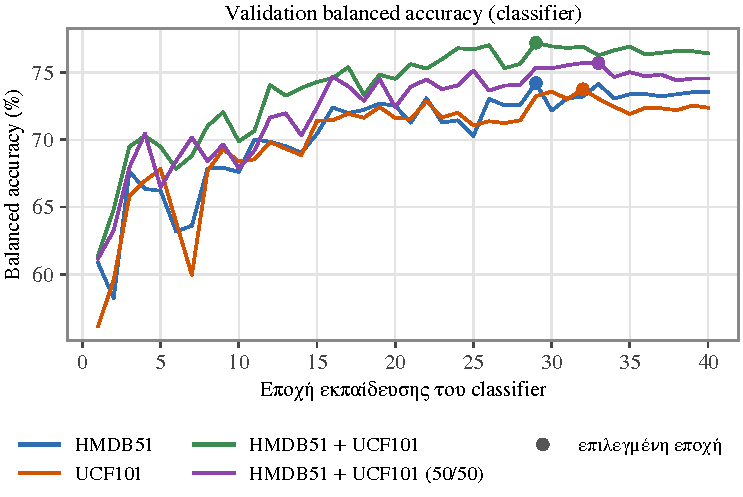
\includegraphics[width=0.72\textwidth]{backbone_kd_data_curves.pdf}
    \caption{Ισορροπημένη ακρίβεια επικύρωσης κατά την εκπαίδευση του
    \tl{attentive classifier} στο \tl{HMDB51}, για \tl{V-JEPA Base}
    \tl{backbones} που αποστάχθηκαν για \(200\) εποχές με διαφορετικά
    δεδομένα. Οι κουκκίδες υποδεικνύουν την εποχή του \tl{checkpoint} που επιλέχθηκε
με βάση τη μέγιστη ισορροπημένη ακρίβεια επικύρωσης.}
    \label{fig:backbone-kd-data-curves}
\end{figure}

Όσον αφορά τα δεδομένα της απόσταξης
(Πίνακας~\ref{tab:backbone-kd-data},
Σχήμα~\ref{fig:backbone-kd-data-curves}), η απόσταξη στο \tl{UCF101}
υπερέχει της απόσταξης στο \tl{HMDB51} κατά \(4{,}58\) ποσοστιαίες
μονάδες στις \(80\) εποχές (Πίνακας~\ref{tab:backbone-kd-exploration}), ενώ στις \(200\) εποχές οι δύο επιδόσεις
είναι πρακτικά ίδιες. Η απόσταξη στο συνδυασμένο σύνολο \tl{HMDB51} + \tl{UCF101} βελτιώνει
την ακρίβεια κατά \(2{,}35\) και \(2{,}74\) ποσοστιαίες μονάδες για την
πλήρη και την ισορροπημένη (\(50/50\)) εκδοχή του, αντίστοιχα, σε σχέση
με την απόσταξη μόνο στο \tl{HMDB51}. Στην ισορροπημένη εκδοχή, οι δύο
συλλογές συνεισφέρουν περίπου τον ίδιο αριθμό βίντεο. Η πλήρης εκδοχή
επιτυγχάνει υψηλότερη ισορροπημένη ακρίβεια επικύρωσης κατά \(1{,}50\)
ποσοστιαίες μονάδες, ωστόσο στο σύνολο ελέγχου οι δύο εκδοχές
επιτυγχάνουν παρόμοια επίδοση, με διαφορά \(0{,}39\) μονάδων, παρότι η
ισορροπημένη χρησιμοποιεί περίπου τα μισά δείγματα.


Η χρήση περισσότερων δεδομένων αυξάνει, ωστόσο, το κόστος της
εκπαίδευσης. Ο χρόνος της απόσταξης εξαρτάται κυρίως από τον όγκο των δεδομένων και
όχι από το μέγεθος του μοντέλου-\tl{student}. Αυτό οφείλεται στο ότι
σε κάθε βήμα, πέρα από το μοντέλο-\tl{student}, εκτελείται και το
σημαντικά μεγαλύτερο μοντέλο-\tl{teacher}, ενώ απαιτείται επίσης η
φόρτωση και η προεπεξεργασία των βίντεο, στάδια κοινά για όλα τα
μοντέλα-\tl{student}. Όπως φαίνεται στον
Πίνακα~\ref{tab:backbone-kd-data}, μία εποχή στον πλήρη συνδυασμό
διαρκεί περίπου \(3{,}6\) φορές περισσότερο από ό,τι στο \tl{HMDB51},
με αποτέλεσμα οι \(200\) εποχές στον πλήρη συνδυασμό να απαιτούν περίπου
\(18\) ώρες σε \tl{GPU NVIDIA A100}, ανεξάρτητα από το μέγεθος του
μοντέλου-\tl{student}.

Συνολικά, η απόσταξη σε διαφορετικό σύνολο δεδομένων από εκείνο της
εκπαίδευσης του \tl{attentive classifier} οδηγεί σε επίδοση παρόμοια με
εκείνη της απόσταξης στο ίδιο το \tl{HMDB51}. Καθώς ο στόχος της
απόσταξης είναι οι αναπαραστάσεις του \tl{teacher}, βίντεο που
προέρχονται από διαφορετικό σύνολο με παρόμοιο περιεχόμενο, εδώ την
αναγνώριση ανθρώπινων ενεργειών, παρέχουν εξίσου χρήσιμη καθοδήγηση στον
\tl{student}. Επομένως, το όφελος της απόσταξης δεν οφείλεται μόνο στο
ότι το \tl{backbone} έχει δει τα ίδια βίντεο με τα οποία εκπαιδεύεται
στη συνέχεια ο \tl{classifier}. Οι υψηλότερες επιδόσεις επιτυγχάνονται με τον συνδυασμό των δύο
συνόλων, γεγονός που υποδεικνύει ότι η μεγαλύτερη ποικιλία των
δεδομένων και η παρουσία βίντεο από το σύνολο αξιολόγησης μπορούν να
συμβάλλουν από κοινού στην επίδοση.

\begin{table}[H]
    \centering
    \caption{Αποτελέσματα στο
    \tl{HMDB51} για τα \tl{V-JEPA Base}, \tl{Small} και \tl{Tiny}, μετά
    από απόσταξη του \tl{backbone} για \(200\) και \(300\) εποχές στο
    \tl{HMDB51} και για \(200\) εποχές στο πλήρες συνδυασμένο σύνολο
    \tl{HMDB51} και \tl{UCF101}.}
    \label{tab:backbone-kd-final-config}
    \small
    \begin{tabular}{lccc}
        \hline
        \textbf{Σύνολο απόσταξης} &
        \begin{tabular}[c]{@{}c@{}}\textbf{Εποχές}\\\textbf{απόσταξης}\end{tabular} &
        \begin{tabular}[c]{@{}c@{}}\textbf{\tl{Val. balanced}}\\\textbf{\tl{accuracy} (\%)}\end{tabular} &
        \begin{tabular}[c]{@{}c@{}}\textbf{\tl{Test}}\\\textbf{\tl{accuracy} (\%)}\end{tabular} \\
        \hline
        \multicolumn{4}{l}{\textit{\tl{V-JEPA Base}}} \\
        \quad\tl{HMDB51}                     & \(200\) & \(74{,}21\) & \(74{,}25\) \\
        \quad\tl{HMDB51}                     & \(300\) & \(75{,}24\) & \(75{,}62\) \\
        \quad\tl{HMDB51} + \tl{UCF101} & \(200\) & \(\mathbf{77{,}20}\) & \(\mathbf{76{,}60}\) \\[6pt]
        \multicolumn{4}{l}{\textit{\tl{V-JEPA Small}}} \\
        \quad\tl{HMDB51}                     & \(200\) & \(66{,}83\) & \(66{,}21\) \\
        \quad\tl{HMDB51}                     & \(300\) & \(68{,}97\) & \(68{,}17\) \\
        \quad\tl{HMDB51} + \tl{UCF101} & \(200\) & \(\mathbf{71{,}12}\) & \(\mathbf{72{,}75}\) \\[6pt]
        \multicolumn{4}{l}{\textit{\tl{V-JEPA Tiny}}} \\
        \quad\tl{HMDB51}                     & \(200\) & \(53{,}62\) & \(50{,}52\) \\
        \quad\tl{HMDB51}                     & \(300\) & \(56{,}58\) & \(54{,}25\) \\
        \quad\tl{HMDB51} + \tl{UCF101} & \(200\) & \(\mathbf{64{,}19}\) & \(\mathbf{61{,}31}\) \\
        \hline
    \end{tabular}
\end{table}

Καθώς η απόσταξη για \(200\) εποχές στο πλήρες συνδυασμένο σύνολο
\tl{HMDB51} και \tl{UCF101} πέτυχε την υψηλότερη ισορροπημένη ακρίβεια
επικύρωσης για το \tl{V-JEPA Base}, επιλέχθηκε ως η τελική διαμόρφωση
και εφαρμόστηκε στη συνέχεια και στα \tl{V-JEPA Small} και \tl{Tiny}
(Πίνακας~\ref{tab:backbone-kd-final-config}). Και στις δύο
αρχιτεκτονικές οδήγησε στην υψηλότερη ακρίβεια ελέγχου μεταξύ των
διαμορφώσεων που εξετάστηκαν, βελτιώνοντάς την κατά \(4{,}58\) και
\(7{,}06\) ποσοστιαίες μονάδες, αντίστοιχα, σε σύγκριση με την απόσταξη
για \(300\) εποχές αποκλειστικά στο \tl{HMDB51}.

\subsection{Διερεύνηση της υπερπροσαρμογής του \tl{attentive classifier}}
\label{subsec:backbone-kd-overfitting}

Παρότι η απόσταξη του \tl{backbone} οδήγησε στις υψηλότερες επιδόσεις
μεταξύ των στρατηγικών που εξετάστηκαν, κατά το δεύτερο στάδιο εκπαίδευσης του \tl{attentive classifier}
παρατηρήθηκε σημαντική απόκλιση μεταξύ της ακρίβειας εκπαίδευσης και
της επίδοσης επικύρωσης του \tl{attentive classifier}. Για τον λόγο αυτό, διερευνήθηκε κατά πόσο η απόκλιση αυτή μπορεί να
περιοριστεί μέσω τεχνικών κανονικοποίησης και διαφορετικών
διαμορφώσεων του \tl{classifier}.

Συγκεκριμένα, εξετάστηκε η εφαρμογή \tl{dropout} στην έξοδο του
\tl{attentive pooler}, με την οποία κάθε στοιχείο του διανύσματος που
προκύπτει μηδενίζεται τυχαία με πιθανότητα \(30\%\), πριν αυτό δοθεί
στο τελικό γραμμικό επίπεδο ταξινόμησης. Εξετάστηκε επίσης η τυχαία
απόρριψη του \(10\%\) των αναπαραστάσεων-\tl{tokens} που εξάγει το
παγωμένο \tl{backbone}, πριν αυτές δοθούν στον \tl{attentive pooler}
κατά την εκπαίδευση (\tl{token dropout}). Επιπλέον, στο \tl{MLP} του \tl{attentive pooler}, όπου η αναπαράσταση
επεκτείνεται σε μεγαλύτερη κρυφή διάσταση και στη συνέχεια επαναφέρεται
στην αρχική, η μετατροπή \(D\rightarrow4D\rightarrow D\)
αντικαταστάθηκε από \(D\rightarrow2D\rightarrow D\), όπου \(D\) είναι η
διάσταση της αναπαράστασης κάθε \tl{token}. Δοκιμάστηκε ακόμη η χρήση σταθμισμένης
\tl{cross-entropy}, με βάρη αντιστρόφως ανάλογα προς τη συχνότητα κάθε
κλάσης στο σύνολο εκπαίδευσης. Τέλος, ο \tl{attentive classifier} αντικαταστάθηκε από έναν απλό
γραμμικό ταξινομητή, ο οποίος δέχεται ως είσοδο τον μέσο όρο των
αναπαραστάσεων-\tl{tokens} του \tl{backbone}.


\begin{table}[H]
    \centering
    \caption{Αποτελέσματα του \tl{attentive classifier} για διαφορετικές
τεχνικές κανονικοποίησης και διαμορφώσεις του \tl{classifier}. Οι
τιμές αντιστοιχούν στην εποχή του \tl{checkpoint} που επιλέχθηκε με
βάση τη μέγιστη ισορροπημένη ακρίβεια επικύρωσης. Σε όλα τα πειράματα
χρησιμοποιείται το \tl{V-JEPA Base} μετά από \(200\) εποχές απόσταξης,
ενώ τόσο η απόσταξη όσο και η εκπαίδευση του \tl{classifier}
πραγματοποιούνται στο \tl{HMDB51}.}
    \label{tab:backbone-kd-overfitting}
    \small
    \begin{tabular}{lccc}
        \hline
        \textbf{Πείραμα} &
        \begin{tabular}[c]{@{}c@{}}\textbf{\tl{Train}}\\\textbf{\tl{accuracy} (\%)}\end{tabular} &
        \begin{tabular}[c]{@{}c@{}}\textbf{\tl{Val. balanced}}\\\textbf{\tl{accuracy} (\%)}\end{tabular} &
        \begin{tabular}[c]{@{}c@{}}\textbf{\tl{Test}}\\\textbf{\tl{accuracy} (\%)}\end{tabular} \\
        \hline
        Αρχική διαμόρφωση                 & \(100\)     & \(\mathbf{74{,}03}\) & \(\mathbf{74{,}25}\) \\
        \hline
        \tl{Dropout} \(0{,}3\)             & \(99{,}93\) & \(71{,}98\) & \(73{,}46\) \\
        \tl{Token dropout} \(0{,}1\)       & \(100\)     & \(73{,}63\) & \(73{,}53\) \\
        \tl{MLP ratio} \(2\)               & \(99{,}72\) & \(74{,}05\) & \(73{,}66\) \\
        Σταθμισμένη \tl{cross-entropy}    & \(99{,}13\) & \(73{,}07\) & \(71{,}57\) \\
        Γραμμικός ταξινομητής             & \(84{,}77\) & \(62{,}63\) & \(62{,}42\) \\
        \hline
    \end{tabular}
\end{table}

Σε όλα σχεδόν τα πειράματα της στρατηγικής, η ακρίβεια εκπαίδευσης στο
\tl{HMDB51} προσεγγίζει το \(100\%\), ενώ η επίδοση επικύρωσης παραμένει
σημαντικά χαμηλότερη. Παρ' όλα αυτά, η ισορροπημένη ακρίβεια
επικύρωσης βρίσκεται κοντά στην ακρίβεια ελέγχου, με μικρές αποκλίσεις
(Πίνακες~\ref{tab:backbone-kd-results} και~\ref{tab:backbone-kd-data}).
Επομένως, παρά την υπερπροσαρμογή, η επίδοση στα δύο σύνολα που δεν
χρησιμοποιούνται στην εκπαίδευση είναι συνεπής, γεγονός που δείχνει ότι
η επιλογή των μοντέλων με βάση το σύνολο επικύρωσης είναι αξιόπιστη.

Οι τεχνικές κανονικοποίησης και οι διαμορφώσεις του \tl{classifier}
που εξετάστηκαν (Πίνακας~\ref{tab:backbone-kd-overfitting}) δεν μείωσαν
ουσιαστικά την απόκλιση ούτε βελτίωσαν την ακρίβεια ελέγχου. Το
\tl{dropout}, το \tl{token dropout}, η μείωση της διάστασης του
\tl{MLP} και η σταθμισμένη \tl{cross-entropy} οδήγησαν σε παρόμοια ή
χαμηλότερη ακρίβεια, ενώ η χρήση γραμμικού ταξινομητή τη μείωσε κατά
\(11{,}83\) ποσοστιαίες μονάδες. Τα αποτελέσματα δείχνουν ότι η υπερπροσαρμογή δεν αντιμετωπίζεται απλώς
με την εφαρμογή των συγκεκριμένων τεχνικών κανονικοποίησης ή με τη
μείωση της χωρητικότητας του \tl{classifier}. Για τον λόγο αυτό,
διερευνήθηκε στη συνέχεια κατά πόσο η συμπεριφορά αυτή σχετίζεται με το
μέγεθος και τα χαρακτηριστικά του συνόλου δεδομένων.

\begin{table}[H]
    \centering
    \caption{Αποτελέσματα του \tl{attentive classifier} για το \tl{V-JEPA Base}
μετά από \(80\) εποχές απόσταξης. Σε κάθε περίπτωση, η απόσταξη και η εκπαίδευση του \tl{classifier}
πραγματοποιούνται στο ίδιο σύνολο δεδομένων, \tl{HMDB51} ή
\tl{UCF101}, το οποίο χρησιμοποιείται και για την επικύρωση και τον
έλεγχο. Οι τιμές αφορούν το \tl{checkpoint}
που επιλέχθηκε με βάση τη μέγιστη ισορροπημένη ακρίβεια επικύρωσης.}
    \label{tab:backbone-kd-overfitting-ucf}
    \small
    \begin{tabular}{llccc}
        \hline
        \begin{tabular}[c]{@{}l@{}}\textbf{Δεδομένα}\\\textbf{απόσταξης}\end{tabular} &
        \begin{tabular}[c]{@{}l@{}}\textbf{Εκπαίδευση}\\\textbf{\tl{classifier}}\end{tabular} &
        \begin{tabular}[c]{@{}c@{}}\textbf{\tl{Train}}\\\textbf{\tl{accuracy} (\%)}\end{tabular} &
        \begin{tabular}[c]{@{}c@{}}\textbf{\tl{Val. balanced}}\\\textbf{\tl{accuracy} (\%)}\end{tabular} &
        \begin{tabular}[c]{@{}c@{}}\textbf{\tl{Test}}\\\textbf{\tl{accuracy} (\%)}\end{tabular} \\
        \hline
        \tl{HMDB51} & \tl{HMDB51}             & \(99{,}97\) & \(66{,}96\) & \(66{,}14\) \\
        \hline
        \tl{UCF101} & \tl{UCF101}             & \(100\)     & \(94{,}33\) & \(93{,}23\) \\
        \tl{UCF101} & \tl{UCF101} (\(2.876\)) & \(100\)     & \(92{,}95\) & \(90{,}91\) \\
        \hline
    \end{tabular}
\end{table}

\begin{figure}[H]
    \centering
    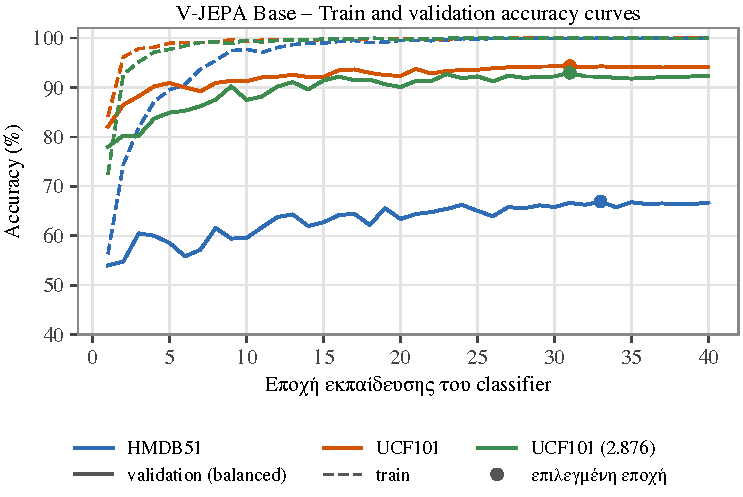
\includegraphics[width=0.72\textwidth]{backbone_kd_ucf_overfitting_curves.pdf}
    \caption{Καμπύλες ακρίβειας εκπαίδευσης (διακεκομμένες γραμμές) και
    ισορροπημένης ακρίβειας επικύρωσης (συνεχείς γραμμές) του
    \tl{attentive classifier} για το \tl{V-JEPA Base}. Για κάθε σύνολο
    δεδομένων, το \tl{backbone} έχει προηγουμένως αποσταχθεί για \(80\)
    εποχές στο ίδιο σύνολο στο οποίο εκπαιδεύεται ο ταξινομητής.
    Εξετάζεται επιπλέον η εκπαίδευση στο \tl{UCF101} με \(2.876\)
    δείγματα, όσα και στο σύνολο εκπαίδευσης του \tl{HMDB51}. Οι
    κουκκίδες υποδεικνύουν την εποχή του επιλεγμένου \tl{checkpoint}.}
    \label{fig:backbone-kd-ucf-overfitting}
\end{figure}

Η σύγκριση των αντίστοιχων διαδικασιών στα δύο σύνολα δεδομένων
(Πίνακας~\ref{tab:backbone-kd-overfitting-ucf},
Σχήμα~\ref{fig:backbone-kd-ucf-overfitting}) αναδεικνύει σημαντική
διαφορά ως προς τη γενίκευση του \tl{attentive classifier}. Όταν τόσο η
απόσταξη του \tl{backbone} όσο και η εκπαίδευση του ταξινομητή
πραγματοποιούνται στο \tl{HMDB51}, η διαφορά μεταξύ της ακρίβειας
εκπαίδευσης και της ισορροπημένης ακρίβειας επικύρωσης ανέρχεται
περίπου στις \(33\) ποσοστιαίες μονάδες. Αντίθετα, στην αντίστοιχη
διαδικασία στο πλήρες \tl{UCF101}, η διαφορά περιορίζεται στις
\(5{,}67\) μονάδες.

Ο μεγαλύτερος όγκος δεδομένων του \tl{UCF101} συμβάλλει θετικά, καθώς η
χρήση του πλήρους συνόλου οδηγεί σε ακρίβεια ελέγχου \(93{,}23\%\),
έναντι \(90{,}91\%\) όταν η εκπαίδευση περιορίζεται σε \(2.876\)
δείγματα. Ωστόσο, ακόμη και με το ίδιο συνολικό πλήθος δειγμάτων με το
\tl{HMDB51}, η διαφορά εκπαίδευσης και επικύρωσης στο \tl{UCF101}
παραμένει μόλις \(7{,}05\) ποσοστιαίες μονάδες. Επομένως, ο μεγαλύτερος
αριθμός δεδομένων βελτιώνει την επίδοση, αλλά δεν εξηγεί από μόνος του
την έντονη υπερπροσαρμογή που εμφανίζεται στο \tl{HMDB51}.

Συνεπώς, η έντονη υπερπροσαρμογή στο \tl{HMDB51} δεν φαίνεται να
οφείλεται αποκλειστικά στο περιορισμένο πλήθος δεδομένων, αλλά συνδέεται
και με τη μεγαλύτερη δυσκολία του συνόλου. Τα βίντεο του \tl{HMDB51} προέρχονται από ποικίλες πηγές, όπως
ψηφιοποιημένες ταινίες και διαδικτυακά βίντεο, και παρουσιάζουν
σημαντικές μεταβολές ως προς την οπτική γωνία, την κίνηση της κάμερας,
την ποιότητα και τον βαθμό ορατότητας του ανθρώπινου σώματος
\cite{kuehne2011hmdb}. Σε συμφωνία με την ερμηνεία αυτή, οι ίδιες μέθοδοι καταγράφουν στη
βιβλιογραφία σημαντικά χαμηλότερες επιδόσεις στο \tl{HMDB51} από ό,τι
στο \tl{UCF101} \cite{tong2022videomae,wang2023videomaev2}.

\section{Συνολική σύγκριση των στρατηγικών απόσταξης}
\label{sec:overall-comparison}

Το Σχήμα~\ref{fig:strategies-comparison} συγκεντρώνει την ακρίβεια
ελέγχου των τριών μοντέλων-\tl{student} για κάθε στρατηγική απόσταξης,
μαζί με τα μοντέλα αναφοράς.

\begin{figure}[H]
    \centering
    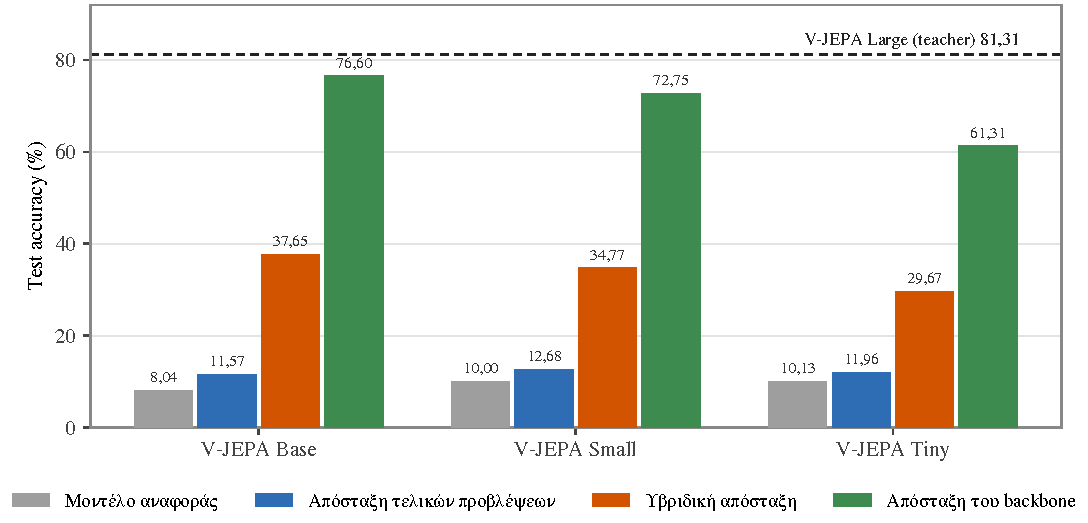
\includegraphics[width=\textwidth]{strategies_comparison.pdf}
    \caption{Ακρίβεια ελέγχου στο \tl{HMDB51} των μοντέλων αναφοράς και
    των μοντέλων-\tl{student} για τις τρεις στρατηγικές απόσταξης, με
    κοινή διαμόρφωση για τις τρεις αρχιτεκτονικές σε κάθε στρατηγική.}
    \label{fig:strategies-comparison}
\end{figure}

Τα υψηλότερα ποσοστά ακρίβειας επιτεύχθηκαν με τη στρατηγική απόσταξης
των αναπαραστάσεων του \tl{backbone}, ακολουθούμενη από την ξεχωριστή
εκπαίδευση του \tl{attentive classifier} πάνω στο παγωμένο αποσταγμένο
\tl{backbone}. Με την καλύτερη πειραματική διαμόρφωση, το
\tl{V-JEPA Base} επιτυγχάνει ακρίβεια \(76{,}60\%\), μόλις \(4{,}71\)
ποσοστιαίες μονάδες χαμηλότερα από το μοντέλο-\tl{teacher}
(\(81{,}31\%\)). Η επίδοση αυτή υπερβαίνει σημαντικά τόσο εκείνη του
αντίστοιχου μοντέλου αναφοράς, το οποίο εκπαιδεύτηκε από την αρχή με
επιβλεπόμενο τρόπο, όσο και τις επιδόσεις που επιτεύχθηκαν με τις δύο
προηγούμενες στρατηγικές απόσταξης.

\begin{table}[H]
    \centering
    \caption{Σύγκριση των μοντέλων-\tl{student} μετά από \(200\) εποχές
απόσταξης του \tl{backbone} στον πλήρη συνδυασμό των \tl{HMDB51} και
\tl{UCF101}. Η μείωση των παραμέτρων
αφορά το σύνολο του \tl{backbone} και του \tl{attentive classifier}
(Πίνακες~\ref{tab:vjepa-model-sizes} και~\ref{tab:vjepa-pooler-sizes}).
Η μέγιστη \tl{VRAM}
μετρήθηκε κατά την αξιολόγηση στο σύνολο ελέγχου με μέγεθος \tl{batch}
\(16\) και ακρίβεια \tl{FP32} σε \tl{GPU NVIDIA A100} και στρογγυλοποιήθηκε στο πλησιέστερο \tl{MiB}. Ο ρυθμός επεξεργασίας
μετρήθηκε στις ίδιες συνθήκες και περιλαμβάνει την ανάγνωση και την
προεπεξεργασία των βίντεο.}
    \label{tab:backbone-kd-final}
    \small
    \setlength{\tabcolsep}{3.5pt}
    \begin{tabular}{lccccc}
        \hline
        \textbf{Μοντέλο} &
        \begin{tabular}[c]{@{}c@{}}\textbf{\tl{Test}}\\\textbf{\tl{accuracy} (\%)}\end{tabular} &
        \begin{tabular}[c]{@{}c@{}}\textbf{Ποσοστό του}\\\textbf{\tl{teacher} (\%)}\end{tabular} &
        \begin{tabular}[c]{@{}c@{}}\textbf{Μείωση}\\\textbf{παραμέτρων (\%)}\end{tabular} &
        \begin{tabular}[c]{@{}c@{}}\textbf{\tl{Peak VRAM}}\\\textbf{(\tl{MiB})}\end{tabular} &
        \begin{tabular}[c]{@{}c@{}}\textbf{\tl{Throughput}}\\\textbf{(\tl{video}/\tl{s})}\end{tabular} \\
        \hline
        \begin{tabular}[c]{@{}l@{}}\tl{V-JEPA Large}\\(\tl{teacher})\end{tabular} & \(81{,}31\) & \(100\)      & ---          & \(2.546\) & \(13{,}59\) \\
        \tl{V-JEPA Base}                 & \(76{,}60\) & \(94{,}2\)   & \(70{,}3\)   & \(1.400\) & \(38{,}39\) \\
        \tl{V-JEPA Small}                & \(72{,}75\) & \(89{,}5\)   & \(92{,}4\)   & \(693\)   & \(55{,}28\) \\
        \tl{V-JEPA Tiny}                 & \(61{,}31\) & \(75{,}4\)   & \(98{,}0\)   & \(402\)   & \(57{,}71\) \\
        \hline
    \end{tabular}
\end{table}

\begin{figure}[H]
    \centering
    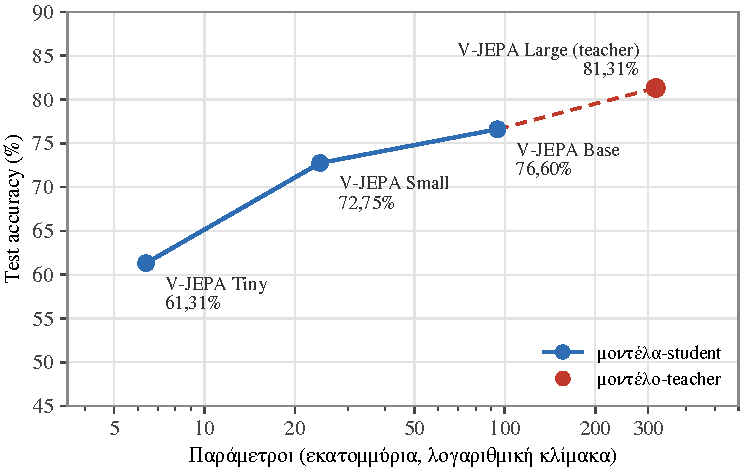
\includegraphics[width=0.72\textwidth]{backbone_kd_accuracy_vs_params.pdf}
    \caption{Ακρίβεια ελέγχου στο \tl{HMDB51} ως προς τον συνολικό αριθμό
    παραμέτρων του \tl{backbone} και του \tl{attentive classifier} για το
    μοντέλο-\tl{teacher} και τα μοντέλα-\tl{student}. Τα \tl{backbones} των
    μοντέλων-\tl{student} έχουν αποσταχθεί για \(200\) εποχές στο πλήρες
    συνδυασμένο σύνολο \tl{HMDB51} και \tl{UCF101}.}
    \label{fig:backbone-kd-accuracy-vs-params}
\end{figure}

Τα αποτελέσματα δείχνουν ότι η ακρίβεια αυξάνεται με το μέγεθος του
μοντέλου-\tl{student}, χωρίς όμως η μείωση των παραμέτρων να προκαλεί
ανάλογη μείωση της επίδοσης. Το \tl{V-JEPA Base} διατηρεί το
\(94{,}2\%\) της ακρίβειας του μοντέλου-\tl{teacher} με \(70{,}3\%\)
λιγότερες παραμέτρους, ενώ η απόκλισή τους περιορίζεται στις
\(4{,}71\) ποσοστιαίες μονάδες. Αυτό δείχνει ότι μεγάλο μέρος της
γνώσης του \tl{teacher} μεταφέρθηκε επιτυχώς στη μικρότερη
αρχιτεκτονική.

Ιδιαίτερα καλή ισορροπία μεταξύ ακρίβειας και μεγέθους επιτυγχάνει το
\tl{V-JEPA Small}, το οποίο διατηρεί το \(89{,}5\%\) της επίδοσης του
\tl{teacher} με \(92{,}4\%\) λιγότερες παραμέτρους, ενώ υστερεί του \tl{V-JEPA Base} μόνο κατά \(3{,}85\)
ποσοστιαίες μονάδες και απαιτεί περίπου \(50\%\) λιγότερη μέγιστη
\tl{VRAM}. Αντίθετα, η μετάβαση στο \tl{V-JEPA Tiny} οδηγεί σε
σημαντικά μεγαλύτερη πτώση της ακρίβειας, κατά \(11{,}44\) ποσοστιαίες
μονάδες σε σχέση με το \tl{V-JEPA Small}. Παρ' όλα αυτά, το
\tl{V-JEPA Tiny} διατηρεί το \(75{,}4\%\) της επίδοσης του
\tl{teacher} με μόλις το \(2\%\) των παραμέτρων του.

Πέρα από τις απαιτήσεις μνήμης, η μείωση του μεγέθους των μοντέλων
επιταχύνει και το \tl{inference}
(Πίνακας~\ref{tab:backbone-kd-final}). Σε σχέση με το
μοντέλο-\tl{teacher}, τα \tl{V-JEPA Base}, \tl{Small} και \tl{Tiny}
επεξεργάζονται περίπου \(2{,}8\), \(4{,}1\) και \(4{,}2\) φορές
περισσότερα βίντεο ανά δευτερόλεπτο, αντίστοιχα. Η επιτάχυνση είναι
σημαντική μέχρι το \tl{V-JEPA Small}, ενώ η διαφορά μεταξύ των
\tl{Small} και \tl{Tiny} είναι περιορισμένη. Για τα μικρότερα μοντέλα,
ο συνολικός χρόνος καθορίζεται κυρίως από την ανάγνωση και την
προεπεξεργασία των βίντεο και σε μικρότερο βαθμό από την εκτέλεση του
ίδιου του μοντέλου.


\begin{figure}[H]
    \centering
    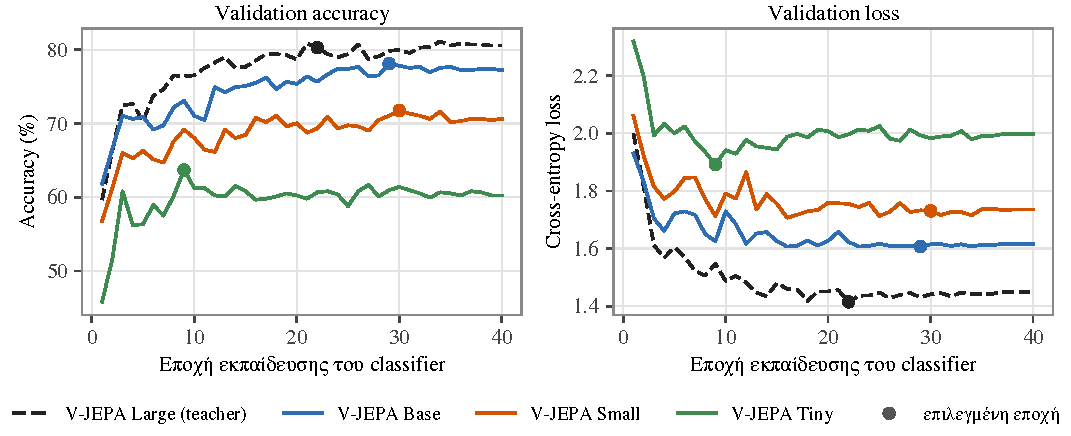
\includegraphics[width=\textwidth]{backbone_kd_teacher_comparison.pdf}
    \caption{Ακρίβεια και απώλεια επικύρωσης κατά την εκπαίδευση του
    \tl{attentive classifier} στο \tl{HMDB51} για το μοντέλο-\tl{teacher}
    και για τα \tl{V-JEPA Base}, \tl{Small} και \tl{Tiny} μετά από
    \(200\) εποχές απόσταξης του \tl{backbone} στο πλήρες συνδυασμένο
    σύνολο \tl{HMDB51} και \tl{UCF101}. Οι κουκκίδες υποδεικνύουν την
    επιλεγμένη εποχή κάθε μοντέλου: για το μοντέλο-\tl{teacher} με βάση
    την ελάχιστη απώλεια επικύρωσης και για τα μοντέλα-\tl{student} με
    βάση τη μέγιστη ισορροπημένη ακρίβεια επικύρωσης.}
    \label{fig:backbone-kd-teacher-comparison}
\end{figure}

Όπως φαίνεται στο Σχήμα~\ref{fig:backbone-kd-teacher-comparison}, η
καμπύλη ακρίβειας επικύρωσης του \tl{V-JEPA Base} ακολουθεί στενά εκείνη
του μοντέλου-\tl{teacher} σε όλη τη διάρκεια της εκπαίδευσης του
\tl{classifier}, με απόκλιση περίπου \(3\) ποσοστιαίων μονάδων μετά τις
πρώτες εποχές. Τα \tl{V-JEPA Small} και \tl{Tiny} παραμένουν σταθερά σε χαμηλότερα
επίπεδα. Ειδικότερα, το \tl{Tiny} φτάνει στη μέγιστη ακρίβειά του ήδη
κατά την 9η εποχή, μετά την οποία η απώλεια επικύρωσης αυξάνεται και η
ακρίβεια μειώνεται.

Συνολικά, το \tl{V-JEPA Base} προσφέρει τη μεγαλύτερη ακρίβεια μεταξύ
των μοντέλων-\tl{student}, το \tl{V-JEPA Small} την καλύτερη ισορροπία
μεταξύ ακρίβειας και μεγέθους, ενώ το \tl{V-JEPA Tiny} τη μεγαλύτερη εξοικονόμηση μνήμης και παραμέτρων.
